\chapter{Nền tảng lý thuyết và công nghệ áp dụng}
\section{Kiến trúc Clean Architecture}
$\indent$ Clean Architecture \cite{clean} được xây dựng trên nền tảng của tư tưởng "độc lập," kết hợp một cách hài hòa với nguyên lý thiết kế hướng đối tượng, trong đó Dependency Inversion là một biểu hiện đặc trưng. Trong bối cảnh này, độc lập có nghĩa là dự án không bị ràng buộc bởi các framework và công cụ được sử dụng trong quá trình kiểm thử.\\

Kiến trúc của Clean Architecture chia thành 4 lớp, mỗi lớp có quy tắc phụ thuộc rõ ràng. Các lớp bên trong được thiết kế để không biết gì về các lớp bên ngoài, thể hiện mối quan hệ phụ thuộc hướng vào bên trong. Clean Architecture giữ cho các phần khác nhau của hệ thống độc lập và linh hoạt, mà không làm suy giảm hiệu suất hay khả năng mở rộng của dự án.

\begin{figure}[H]
    \centering
    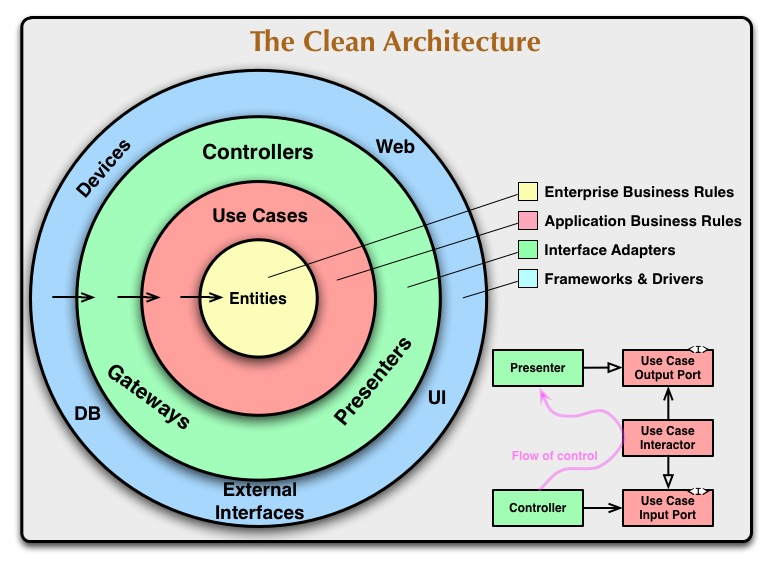
\includegraphics[width=0.8\linewidth]{Images/clean.png}
    \vspace{1em}
    \caption{Minh hoạ Clean Architecture, nguồn \cite{clean}}
    \label{fig:clean}
\end{figure}

Ở mức độ chi tiết, Thực thể đóng vai trò như những yếu tố cơ bản trong kiến trúc, đóng gói quy tắc kinh doanh toàn diện. Dù có dạng đối tượng hoặc là cấu trúc dữ liệu và chức năng, thực thể không quan tâm đến ứng dụng cụ thể nào đang sử dụng chúng. Trong khi đó, Lớp Use Cases chứa quy tắc kinh doanh cụ thể cho ứng dụng và đảm bảo luồng dữ liệu giữa các thực thể.\\

Interface Adapters đóng vai trò như trung gian, chuyển đổi dữ liệu giữa định dạng thuận tiện nhất cho Use Cases và Thực thể và định dạng thuận tiện nhất cho đơn vị bên ngoài như cơ sở dữ liệu hoặc web. Cuối cùng, lớp Frameworks và Drivers chứa các công cụ và chi tiết cấp thấp nhất, như cơ sở dữ liệu và framework web, với chức năng chính là đóng vai trò như một đường ống.\\

Quy tắc phụ thuộc luôn được duy trì, giúp tăng cường trừu tượng hóa theo hướng vòng tròn bên trong. Mỗi lớp giữ vai trò của một hộp chứa độc lập, giúp duy trì sự cân bằng giữa linh hoạt và sự kiểm soát trong thiết kế kiến trúc Clean Architecture.

\section{Design pattern: DI and builder}

$\indent$Trong thế giới phát triển phần mềm hiện đại, việc sử dụng Design Pattern không chỉ là một xu hướng mà còn là một chiến lược quan trọng để tạo ra mã nguồn dễ bảo trì và linh hoạt. Hai mô hình quan trọng, Dependency Injection (DI) và Builder Pattern, là những "công cụ" quan trọng trong "hộp công cụ" của các nhà phát triển giúp tối ưu hóa việc quản lý các thành phần của hệ thống và cung cấp khả năng linh hoạt đáng kể trong việc xây dựng đối tượng phức tạp.

\section*{Dependency Injection (DI):}

$\indent$ DI \cite{di} là một design pattern tập trung vào việc giảm sự phụ thuộc giữa các thành phần của hệ thống, giúp tăng tính linh hoạt và kiểm soát. Thay vì các đối tượng tạo ra và quản lý chính nó, DI chuyển trách nhiệm này đến bên ngoài, thường là một hệ thống quản lý phụ thuộc (dependency container). Điều này giúp giảm độ kết dính giữa các thành phần, làm cho mã nguồn dễ bảo trì và mở rộng hơn. Hơn nữa, DI thúc đẩy việc tái sử dụng mã nguồn, vì các đối tượng không phụ thuộc trực tiếp vào cách chúng được tạo ra.

\begin{figure}[h]
    \centering
    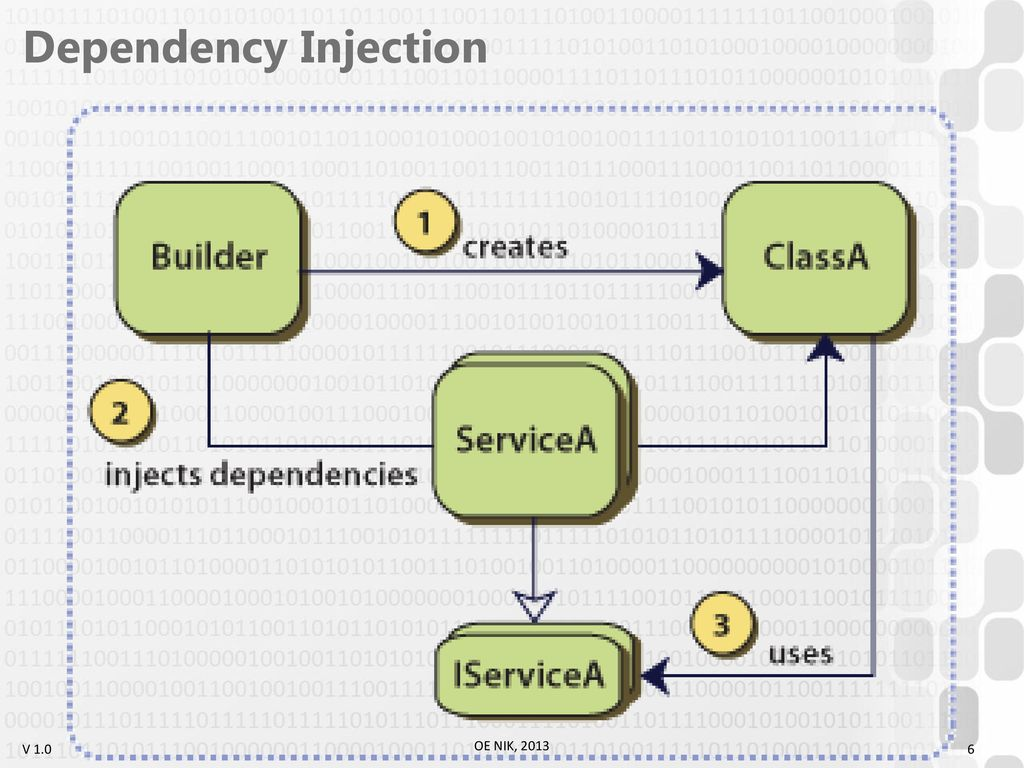
\includegraphics[width=0.6\linewidth]{Images/DI.png}
    \vspace{1em}
    \caption{Dependency Injection}
    
\end{figure}
\newpage
\section*{Builder Pattern:}

$\indent$ Builder Pattern \cite{builder} tập trung vào việc xây dựng đối tượng phức tạp, giúp tách rời quá trình xây dựng và biểu diễn. Thay vì sử dụng nhiều constructor hoặc phương thức khởi tạo, Builder Pattern cung cấp một cách linh hoạt và tự nhiên để xây dựng đối tượng bằng cách sử dụng một builder object. Điều này không chỉ làm cho mã nguồn dễ đọc hơn mà còn giúp quản lý các tham số xây dựng, đặc biệt là khi có nhiều tùy chọn. Builder Pattern thường được sử dụng để xây dựng các đối tượng không thay đổi và không có sự thay đổi trạng thái, giúp giảm lỗi và làm tăng khả năng kiểm thử.

\begin{figure}[h]
    \centering
    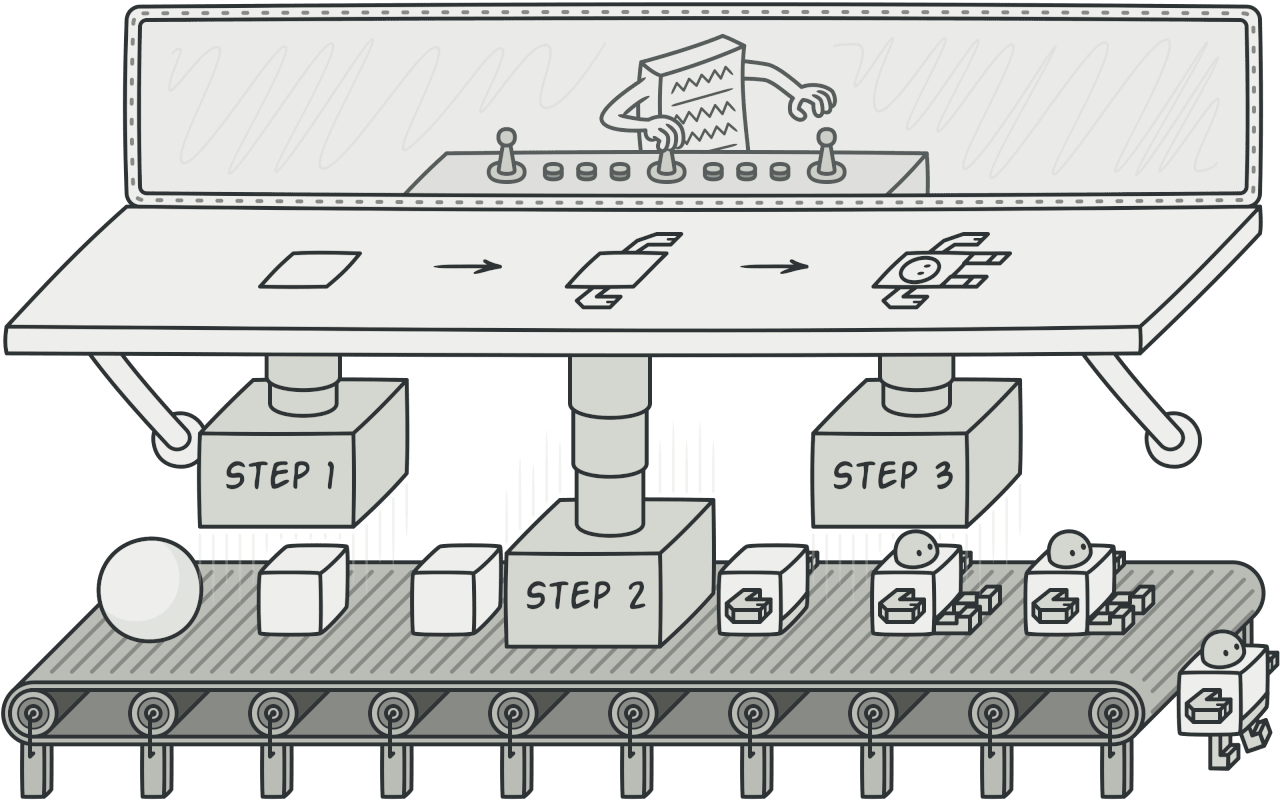
\includegraphics[width=\linewidth]{Images/builder.png}
    \vspace{1em}
    \caption{Builder cho phép xây dựng các đối tượng phức tạp theo từng bước}
    
\end{figure}

\section*{Tích Hợp DI và Builder Pattern:}

$\indent$ Khi kết hợp DI và Builder Pattern, chúng ta có thể tận dụng sức mạnh của cả hai mô hình để tạo ra hệ thống linh hoạt, dễ bảo trì, và có thể mở rộng một cách dễ dàng. Dependency Injection giảm sự phụ thuộc, trong khi Builder Pattern giúp quản lý quá trình xây dựng các đối tượng phức tạp. Sự kết hợp này làm cho mã nguồn dễ đọc, dễ kiểm thử, và giảm thiểu các vấn đề liên quan đến thiết kế và xây dựng.\\

Bằng cách tận dụng sự mạnh mẽ của cả Dependency Injection và Builder Pattern, chúng ta có thể xây dựng các hệ thống linh hoạt và dễ bảo trì, đồng thời giảm thiểu rủi ro về lỗi và tăng tính mở rộng của mã nguồn.

\section{Front-end}
\subsection{Next.js với TypeScript}
$\indent$ Next.js \cite{nextjs} là một framework React mã nguồn mở được phát triển bởi Vercel, nhằm cung cấp một giải pháp toàn diện cho việc xây dựng ứng dụng web hiện đại. Next.js kế thừa tất cả ưu điểm của React và bổ sung thêm nhiều tính năng mạnh mẽ. 

Next.js sử dụng cách tiếp cận "page-based routing" kết hợp với "component-based" của React để xây dựng giao diện. Điều này cho phép tổ chức cấu trúc ứng dụng một cách trực quan và hiệu quả, đồng thời vẫn giữ được khả năng tái sử dụng và modular hóa cao của các component. Cách tiếp cận này giúp tách biệt logic và giao diện, dễ dàng quản lý và bảo trì mã nguồn, đồng thời tạo ra một kiến trúc ứng dụng rõ ràng và dễ mở rộng.

Một trong những tính năng nổi bật của Next.js là khả năng Server-Side Rendering (SSR) và Static Site Generation (SSG). SSR giúp cải thiện đáng kể thời gian tải trang đầu tiên và tối ưu hóa SEO, trong khi SSG cho phép tạo ra các trang tĩnh tại thời điểm build, giúp tăng tốc độ và giảm tải cho server. Next.js cũng hỗ trợ Incremental Static Regeneration (ISR), cho phép cập nhật từng phần của trang tĩnh mà không cần phải build lại toàn bộ site.

Next.js tích hợp sẵn nhiều tính năng quan trọng như code splitting, lazy loading, và tối ưu hóa hình ảnh. Điều này giúp cải thiện hiệu suất ứng dụng một cách đáng kể mà không cần cấu hình phức tạp.

Khi kết hợp Next.js với TypeScript, ta có thể tận dụng tất cả lợi ích của việc kiểm tra kiểu tĩnh và lập trình hướng đối tượng mạnh mẽ. TypeScript giúp phát hiện lỗi trong quá trình biên dịch và cung cấp các tính năng gỡ lỗi thông minh, tăng tính ổn định và độ tin cậy của ứng dụng \cite{typescript}.

Việc sử dụng TypeScript với Next.js còn mang lại lợi ích trong việc quản lý trạng thái và props của components. TypeScript cho phép xác định các kiểu dữ liệu chính xác cho trạng thái, props, và các API routes của Next.js, giúp tạo ra mã nguồn dễ đọc, dễ hiểu và dễ bảo trì. Điều này đặc biệt hữu ích trong các dự án lớn và phức tạp.

Next.js cũng cung cấp API Routes, cho phép xây dựng API serverless một cách dễ dàng. Kết hợp với TypeScript, ta có thể tạo ra các API an toàn về kiểu dữ liệu và dễ dàng tích hợp với phần front-end của ứng dụng.

Tóm lại, Next.js kết hợp với TypeScript là một công cụ mạnh mẽ cho phát triển ứng dụng web hiện đại. Với khả năng SSR, SSG, ISR, hiệu suất cao, kiến trúc dựa trên pages và components, tính năng mạnh mẽ của TypeScript và sự hỗ trợ từ cộng đồng, Next.js giúp tạo ra các ứng dụng web linh hoạt, có hiệu suất cao, dễ bảo trì và đáng tin cậy.

\begin{figure}[h]
    \centering
    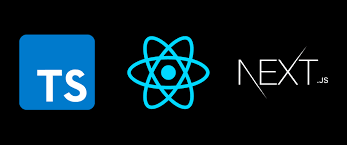
\includegraphics[width=0.5\linewidth]{Images/nextjs.png}
    \vspace{1em}
    \caption{Next.js và Typescript}
    
\end{figure}
\newpage
\subsection{Mantine}
$\indent$ Mantine \cite{mantine} là một thư viện UI React mã nguồn mở, cung cấp các thành phần giao diện đẹp mắt, dễ sử dụng và linh hoạt. Nó cung cấp một tập hợp các thành phần giao diện hiện đại, từ các nút, biểu mẫu và bảng cho đến các thanh trượt, menu và hộp thoại. Điều này giúp tạo ra giao diện thân thiện với người dùng, hiệu quả và đồng nhất trên toàn bộ ứng dụng.\\

Một trong những điểm mạnh của Mantine là tính tùy chỉnh cao. Nó không chỉ cung cấp các thành phần giao diện sẵn có, mà còn cho phép người phát triển tùy chỉnh chúng dựa trên nhu cầu cụ thể. Điều này đảm bảo rằng giao diện cuối cùng sẽ phù hợp với mục tiêu thiết kế và mong muốn của người dùng.\\

Ngoài ra, Mantine còn cung cấp một bộ tài liệu phong phú và chi tiết, gồm hướng dẫn sử dụng, ví dụ mẫu và hướng dẫn thiết kế. Điều này giúp người phát triển nhanh chóng làm quen với Ant Design và tận dụng tối đa các tính năng mạnh mẽ của nó.\\

Mantine là một lựa chọn lý tưởng để xây dựng giao diện người dùng chất lượng và dễ sử dụng trong các dự án phát triển phần mềm. Với tính tương thích, tích hợp dễ dàng, tính tùy chỉnh cao, Mantine là lựa chọn thích hợp đối với công cụ phát triển giao diện người dùng.

\begin{figure}[h]
    \centering
    
\includegraphics[width=0.5\linewidth]{Images/matine.png}
    \vspace{1em}
    \caption{Mantine}
    
\end{figure}

\section{Back-end và Database}
\subsection{ASP.NET Core và Entity Framework (EF) Core}

$\indent$ ASP.NET Core \cite{asp}là một framework phát triển ứng dụng web mạnh mẽ được phát triển bởi Microsoft. Nó cung cấp một nền tảng cho việc xây dựng các ứng dụng web đa dạng và mạnh mẽ bằng cách sử dụng ngôn ngữ lập trình C\#.\\

Entity Framework(EF) Core \cite{ef} là một ORM (Object-Relational Mapping) framework cũng do Microsoft phát triển, giúp tương tác và quản lý cơ sở dữ liệu trong ứng dụng. Nó giúp lập trình viên làm việc với dữ liệu cơ sở dữ liệu bằng cách sử dụng đối tượng và cung cấp một lớp trừu tượng giúp ẩn đi các chi tiết về cơ sở dữ liệu thực tế.\\ 

Khi kết hợp sử dụng ASP.NET Core và Entity Framework Core, người phát triển có thể xây dựng các ứng dụng web mạnh mẽ và dễ dàng quản lý cơ sở dữ liệu. Thông qua Entity Framework Core, dữ liệu được quản lý trong các đối tượng .NET, giúp giảm thiểu việc phải viết các câu truy vấn SQL trực tiếp. Thêm vào đó, ASP.NET Core cung cấp nền tảng cho việc xây dựng các giao diện người dùng tương tác, cho phép người dùng tương tác với dữ liệu được quản lý bởi Entity Framework Core.\\

Tóm lại, sự kết hợp giữa ASP.NET Core và Entity Framework Core cung cấp cho các nhà phát triển một cách tiếp cận toàn diện để xây dựng ứng dụng web chất lượng cao với khả năng tương tác với dữ liệu hiệu quả.

\begin{figure}[H]
    \centering
    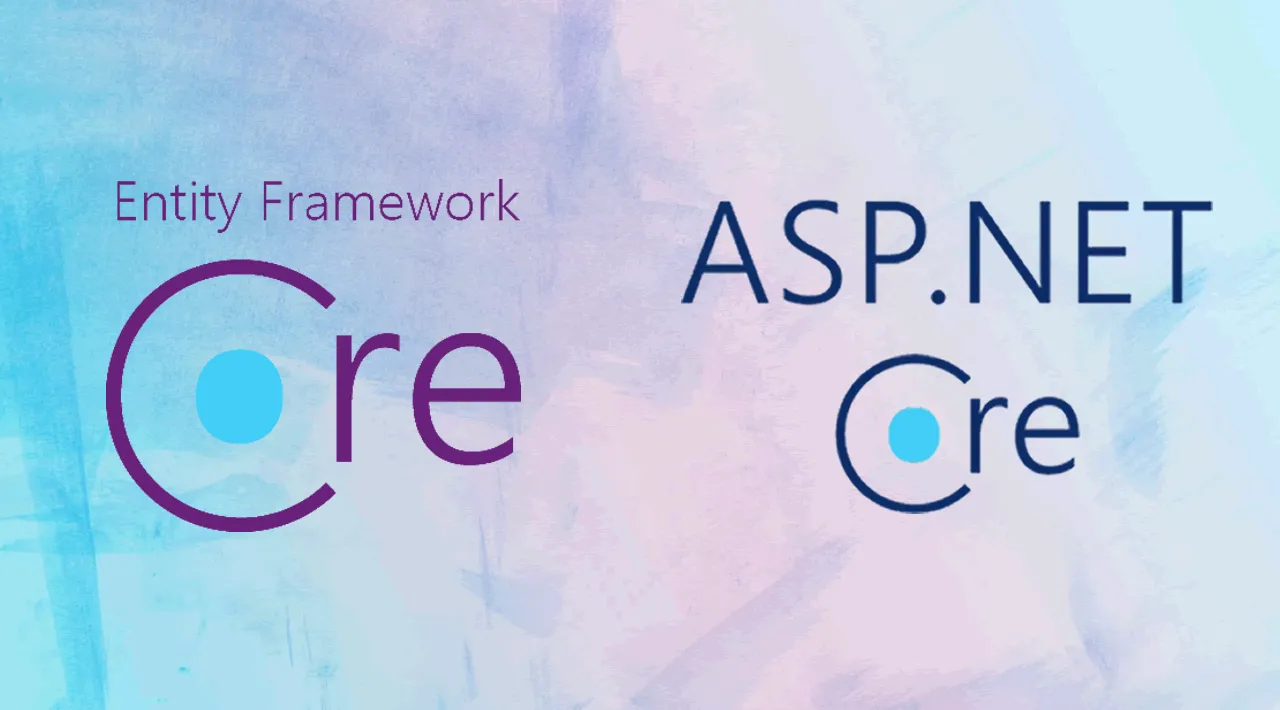
\includegraphics[width=0.55\linewidth]{Images/asp-ef.png}
    \vspace{1em}
    \caption{EF Core và ASP.NET Core}
    
\end{figure}


\subsection{PostgreSQL Database}
$\indent$ PostgreSQL Database \cite{postgreSql} là một hệ quản trị cơ sở dữ liệu quan hệ mã nguồn mở mạnh mẽ và đáng tin cậy, được phát triển bởi cộng đồng PostgreSQL Global Development Group. Với hơn 30 năm phát triển, PostgreSQL đã trở thành một trong những lựa chọn hàng đầu cho các ứng dụng yêu cầu độ tin cậy cao, tính toàn vẹn dữ liệu, và khả năng xử lý khối lượng lớn.

Dự án đã tận dụng sức mạnh của PostgreSQL thông qua dịch vụ Neon, một nền tảng cung cấp PostgreSQL trên cloud. Neon cung cấp một giải pháp serverless, cho phép tập trung vào việc phát triển ứng dụng mà không cần lo lắng về việc quản lý cơ sở hạ tầng. Điều này giúp tối ưu hóa chi phí vận hành và tăng tính linh hoạt cho hệ thống.

Tính năng ACID (Atomicity, Consistency, Isolation, Durability) của PostgreSQL đảm bảo tính toàn vẹn dữ liệu cao, điều này đặc biệt quan trọng đối với các ứng dụng yêu cầu độ tin cậy cao như hệ thống của nhóm. Ngoài ra, PostgreSQL còn cung cấp các tính năng nâng cao như partitioning, replication, và full-text search, giúp tối ưu hóa hiệu suất và khả năng mở rộng của hệ thống.

Về mặt bảo mật, PostgreSQL cung cấp nhiều lớp bảo vệ, bao gồm xác thực mạnh mẽ, mã hóa dữ liệu, và kiểm soát truy cập chi tiết. Khi kết hợp với các tính năng bảo mật của Neon, có thể đảm bảo rằng dữ liệu của người dùng luôn được bảo vệ ở mức cao nhất.

PostgreSQL cũng nổi tiếng với khả năng mở rộng và hiệu suất cao. Nó có thể xử lý hàng triệu bản ghi một cách hiệu quả, đồng thời hỗ trợ các truy vấn phức tạp và các giao dịch đồng thời. Điều này cho phép ứng dụng phục vụ số lượng lớn người dùng mà không gặp vấn đề về hiệu suất.

Cuối cùng, việc sử dụng PostgreSQL trên nền tảng Neon cho phép tận dụng các tính năng như sao lưu tự động, khôi phục điểm thời gian, và scaling tự động. Điều này giúp đảm bảo tính khả dụng cao và khả năng phục hồi nhanh chóng trong trường hợp xảy ra sự cố.

Tóm lại, việc lựa chọn PostgreSQL trên nền tảng Neon đã cung cấp một giải pháp cơ sở dữ liệu mạnh mẽ, linh hoạt và đáng tin cậy. Nó không chỉ đáp ứng các yêu cầu hiện tại của dự án mà còn cung cấp nền tảng vững chắc cho sự phát triển trong tương lai.

\begin{figure}[H]
    \centering
    
\includegraphics[width=0.8\linewidth]{Images/tech_database.png}
    \vspace{1em}
    \caption{PostgreSQL Service}
    
\end{figure}

\subsection{Redis}
$\indent$ Redis \cite{redis} là một hệ thống lưu trữ cấu trúc dữ liệu key-value trong bộ nhớ, được sử dụng rộng rãi như một giải pháp caching hiệu quả. Nó được phát triển như một dự án mã nguồn mở và hỗ trợ nhiều cấu trúc dữ liệu như chuỗi, hash, danh sách, tập hợp và sorted sets. Redis nổi tiếng với hiệu suất cao và khả năng xử lý hàng triệu yêu cầu mỗi giây.

Redis cung cấp nhiều ưu điểm quan trọng cho dự án. Đầu tiên, tốc độ xử lý của Redis rất nhanh do lưu trữ dữ liệu trong bộ nhớ RAM, cho phép truy xuất dữ liệu với độ trễ cực thấp. Thứ hai, Redis hỗ trợ đa dạng cấu trúc dữ liệu, giúp lưu trữ và truy xuất dữ liệu một cách linh hoạt. Thứ ba, Redis có khả năng persistence, cho phép lưu dữ liệu vào ổ đĩa, đảm bảo tính bền vững của dữ liệu. Ngoài ra, Redis dễ dàng mở rộng theo chiều ngang với các cụm Redis và có thư viện hỗ trợ cho hầu hết các ngôn ngữ lập trình phổ biến.

Việc sử dụng Redis trong dự án giúp tối ưu hóa hiệu suất ứng dụng bằng cách giảm thời gian truy xuất dữ liệu, giảm tải cho cơ sở dữ liệu chính và cải thiện trải nghiệm người dùng với thời gian phản hồi nhanh hơn. Redis đặc biệt hữu ích trong việc lưu trữ các dữ liệu tạm thời như phiên đăng nhập, kết quả tính toán phức tạp, và dữ liệu được truy cập thường xuyên.
\begin{figure}[H]
    \centering
    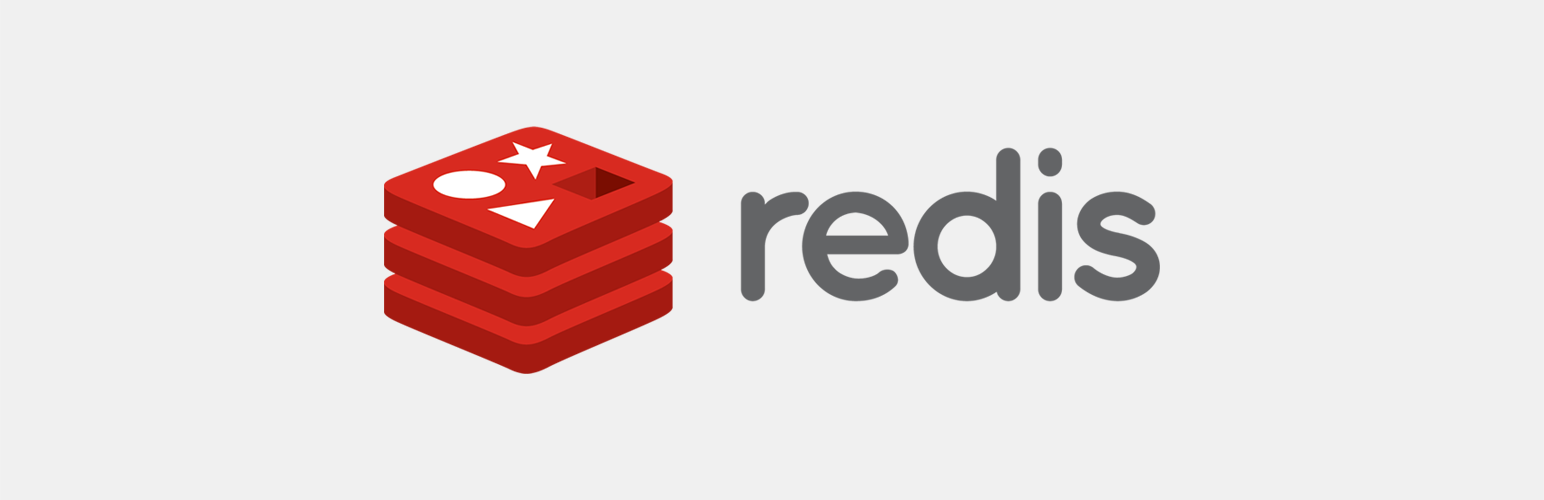
\includegraphics[width=0.8\linewidth]{Images/redis.png}
    \vspace{1em}
    \caption{Redis}
    
\end{figure}

\subsection{Cloudinary}
$\indent$ Cloudinary \cite{cloudinary} là một nền tảng quản lý hình ảnh và video trên đám mây, cung cấp giải pháp toàn diện cho việc tải lên, lưu trữ, tối ưu hóa, và phân phối nội dung đa phương tiện. Nền tảng này được thiết kế để giúp các nhà phát triển và doanh nghiệp quản lý hiệu quả tài sản đa phương tiện của họ, đồng thời cung cấp các công cụ mạnh mẽ để xử lý và phân phối nội dung.

Lựa chọn Cloudinary cho quản lý hình ảnh trong dự án mang lại nhiều lợi ích đáng kể. Đầu tiên, Cloudinary cung cấp khả năng tự động tối ưu hóa hình ảnh, cân bằng giữa chất lượng và kích thước file, giúp tăng tốc độ tải trang. Thứ hai, nền tảng này cho phép biến đổi hình ảnh linh hoạt thông qua URL, bao gồm thay đổi kích thước, cắt, xoay và áp dụng các hiệu ứng. Thứ ba, Cloudinary sử dụng CDN (Content Delivery Network) để phân phối nội dung nhanh chóng trên toàn cầu, cải thiện trải nghiệm người dùng ở mọi vị trí địa lý.

Bên cạnh đó, Cloudinary cung cấp nhiều tùy chọn bảo mật như chữ ký URL và hạn chế truy cập, đảm bảo an toàn cho tài sản đa phương tiện. Nền tảng này cũng có giao diện quản lý trực quan, dễ sử dụng cho việc tổ chức và tìm kiếm tài sản. Đặc biệt, Cloudinary cung cấp SDK và API cho nhiều ngôn ngữ lập trình và framework phổ biến, giúp tích hợp dễ dàng vào dự án. Tóm lại, bằng cách sử dụng Cloudinary, dự án có thể tập trung vào việc phát triển các tính năng cốt lõi mà không cần lo lắng về việc quản lý, tối ưu hóa và phân phối hình ảnh, đồng thời đảm bảo rằng nội dung đa phương tiện được xử lý một cách chuyên nghiệp và hiệu quả.

\begin{figure}[H]
    \centering
    
\includegraphics[width=0.3\linewidth]{Images/cloudinary.png}
    \vspace{1em}
    \caption{Cloudinary}
    
\end{figure}

\section{Deploy}
\subsection{Vercel}
$\indent$ Vercel \cite{vercel} là một nền tảng triển khai và lưu trữ trang web, ứng dụng Front-end được phát triển bởi Vercel, Inc. (trước đây là Zeit). Nền tảng này được thiết kế đặc biệt để triển khai các ứng dụng web hiện đại và tĩnh dựa trên các framework như React, Next.js, Vue.js và Nuxt.js.\\

Với Vercel, có thể dễ dàng triển khai mã nguồn thông qua quy trình CI/CD tích hợp sẵn. Nền tảng này tự động xây dựng, triển khai và cung cấp các bản xem trước cho mỗi lần push code lên Git. Vercel cũng cung cấp các tính năng như phân phối nội dung toàn cầu thông qua mạng CDN, quản lý các bản triển khai, tích hợp các dịch vụ bên thứ ba và tự động hóa quy trình build/deploy.\\

Một trong những lợi ích chính của Vercel là nó cho phép tập trung vào việc xây dựng ứng dụng mà không cần phải lo lắng về việc quản lý cơ sở hạ tầng triển khai. Vercel xử lý tất cả các nhiệm vụ liên quan đến triển khai, bảo mật và mở rộng, giúp gia tăng năng suất và tập trung vào phát triển tính năng.
\begin{figure}[h]
    \centering
    
\includegraphics[width=0.5\linewidth]{Images/vercel.png}
    \vspace{1em}
    \caption{Vercel}
\end{figure}
\subsection{Render}
Render \cite{render} là một nền tảng đám mây hiện đại được thiết kế để triển khai và quản lý các ứng dụng web, API, cơ sở dữ liệu và các dịch vụ backend khác. Nền tảng này cung cấp một môi trường đơn giản nhưng mạnh mẽ cho việc triển khai các ứng dụng từ nhiều ngôn ngữ lập trình và framework khác nhau, bao gồm Node.js, Python, Ruby, Go và các ứng dụng Docker. Render tự động hóa nhiều quy trình phức tạp trong việc triển khai và quản lý ứng dụng, giúp phát triển tập trung vào việc viết mã thay vì lo lắng về cơ sở hạ tầng.

Một trong những ưu điểm chính của Render là khả năng tích hợp CI/CD (Continuous Integration/Continuous Deployment) liền mạch. Nền tảng này tự động phát hiện các thay đổi trong kho lưu trữ Git và triển khai các bản cập nhật, giúp quy trình phát triển và triển khai trở nên nhanh chóng và hiệu quả. Render cũng cung cấp tính năng tự động mở rộng, cho phép ứng dụng dễ dàng đáp ứng với lưu lượng truy cập tăng đột biến mà không cần can thiệp thủ công. Ngoài ra, Render còn cung cấp chứng chỉ SSL miễn phí, bảo mật DDoS và các tính năng bảo mật khác để đảm bảo an toàn cho ứng dụng.

Render đặc biệt phù hợp cho việc triển khai backend vì nó cung cấp môi trường có thể tùy chỉnh cao, hỗ trợ nhiều loại cơ sở dữ liệu và dịch vụ phụ trợ. Nền tảng này cho phép dễ dàng quản lý các biến môi trường, theo dõi logs và giám sát hiệu suất ứng dụng. Với giao diện người dùng trực quan và API mạnh mẽ, Render giúp đơn giản hóa quy trình quản lý và duy trì ứng dụng backend. Tóm lại, Render cung cấp một giải pháp toàn diện cho việc triển khai và quản lý backend, cho phép nhóm tập trung vào việc xây dựng tính năng và cải thiện ứng dụng mà không phải lo lắng về các vấn đề phức tạp của cơ sở hạ tầng.

\begin{figure}[h]
    \centering
    
\includegraphics[width=0.5\linewidth]{Images/render.jpeg}
    \vspace{1em}
    \caption{Render}
\end{figure}
